\documentclass[a4paper,17pt]{extarticle}


    \usepackage[sfdefault, condensed]{roboto} % police d'écriture plus moderne
\usepackage[french]{babel} % francisation
\usepackage[parfill]{parskip} %suppression indentation

\usepackage{fancyhdr}
\usepackage{multicol}

% figure non flotantes
\usepackage{float}
\let\origfigure\figure
\let\endorigfigure\endfigure
\renewenvironment{figure}[1][2] {
    \expandafter\origfigure\expandafter[H]
} {
    \endorigfigure
}

% mois/année
\usepackage{datetime}
\newdateformat{monthyeardate}{%
  \monthname[\THEMONTH] \THEYEAR}

% couleurs perso
\usepackage[table]{xcolor}
\definecolor{deepblue}{rgb}{0.3,0.3,0.8}
\definecolor{darkblue}{rgb}{0,0,0.3}
\definecolor{deepred}{rgb}{0.6,0,0}
\definecolor{iremred}{RGB}{204,35,50}
\definecolor{deepgreen}{rgb}{0,0.6,0}
\definecolor{backcolor}{rgb}{0.98,0.95,0.95}
\definecolor{grisClair}{rgb}{0.95,0.95,0.95}
\definecolor{orangeamu}{RGB}{250,178,11}
\definecolor{noiramu}{RGB}{35,31,32}
\definecolor{bleuamu}{RGB}{20,118,198}
\definecolor{bleuamudark}{RGB}{15,90,150}
\definecolor{cyanamu}{RGB}{77,198,244}


\usepackage{/home/bouscadilla/Documents/Code/nbconvert/template/latex/pdf_solution/xeboiboites}
%
% exemple
\newbreakabletheorem[
    small box style={fill=deepblue!90,draw=deepblue!15, rounded corners,line width=1pt},%
    big box style={fill=deepblue!5,draw=deepblue!15,thick,rounded corners,line width=1pt},%
    headfont={\color{white}\bfseries}
        ]{exemple}{Exemple}{}%{counterCo}
%
% remarque
\newbreakabletheorem[
    small box style={draw=ansi-green-intense!100,line width=2pt,fill=ansi-green-intense!0,rounded corners,decoration=penciline, decorate},%
	big box style={color=ansi-green-intense!90,fill=ansi-green-intense!10,thick,decoration={penciline},decorate},
    broken edges={draw=ansi-green-intense!90,thick,fill=orange!20!black!5, decoration={random steps, segment length=.5cm,amplitude=1.3mm},decorate},%
    other edges={decoration=penciline,decorate,thick},%
    headfont={\color{ansi-green-intense}\large\scshape\bfseries}
    ]{remarque}{Remarque}{}%{counterCa}
%
% formule (sans titre)
\newboxedequation[%
    big box style={fill=cyanamu!10,draw=cyanamu!100,thick,decoration=penciline,decorate}]%
    {form}
%
% Réponse
\newbreakabletheorem[
    small box style={fill=bleuamu!100, draw=bleuamu!60, line width=1pt,rounded corners,decorate},%
    big box style={fill=bleuamu!10,draw=bleuamu!30,thick,rounded corners,decorate},
    headfont={\color{white}\large\scshape\bfseries}
        ]{reponse}{Correction}{}
%

%
% À retenir
%\newbreakabletheorem[
%    small box style={fill=deepred!100, draw=deepred!80, line width=1pt,rounded corners,decorate},%
%    big box style={fill=deepred!10,draw=deepred!50,thick,rounded corners,decorate},
%    headfont={\color{white}\large\scshape\bfseries}
%        ]{retenir}{À retenir}{}
%
\newboxedequation[%
    big box style={fill=deepred!10,draw=deepred!0,thick,decoration=penciline,decorate}]%
    {retenir}



% astuce
\newspanning[
    image=/home/bouscadilla/Documents/Code/nbconvert/template/latex/pdf_solution/fig-idee,headfont=\bfseries,
    spanning style={very thick,decoration=penciline,decorate}
    ]{astuce}{Astuce}{}
%
% activité

\newcounter{counterCa}
\newbreakabletheorem[
    small box style={draw=orangeamu!100,line width=2pt,fill=orangeamu!100,rounded corners,decoration=penciline, decorate},%
	big box style={color=orangeamu!100,fill=orangeamu!5,thick,decoration={penciline},decorate},
    broken edges={draw=orangeamu!100,thick,fill=orangeamu!100, decoration={random steps, segment length=.5cm,amplitude=1.3mm},decorate},%
    other edges={decoration=penciline,decorate,thick},%
    headfont={\color{white}\large\scshape\bfseries}
    ]{activite}{\adjustimage{height=1cm, valign=m}{/home/bouscadilla/Documents/Code/nbconvert/template/latex/pdf_solution/papier_eleve_investigation.png}%
    Activité}{counterCa}
%   
%   environnement élève
%
\newenvironment{eleve}%
%{\begin{activite}\large\\} % écrire plus gros
{\begin{activite}\color{noiramu}\\[-0.5cm]}
{\end{activite}}

\newenvironment{formule}%
%{\begin{activite}\large\\} % écrire plus gros
{\begin{form}\color{bleuamu}}
{\end{form}}


\usepackage[breakable]{tcolorbox}
    \usepackage{parskip} % Stop auto-indenting (to mimic markdown behaviour)
    
    \usepackage{iftex}
    \ifPDFTeX
    	\usepackage[T1]{fontenc}
    	\usepackage{mathpazo}
    \else
    	\usepackage{fontspec}
    \fi

    % Basic figure setup, for now with no caption control since it's done
    % automatically by Pandoc (which extracts ![](path) syntax from Markdown).
    \usepackage{graphicx}
    % Maintain compatibility with old templates. Remove in nbconvert 6.0
    \let\Oldincludegraphics\includegraphics
    % Ensure that by default, figures have no caption (until we provide a
    % proper Figure object with a Caption API and a way to capture that
    % in the conversion process - todo).
    \usepackage{caption}
    \DeclareCaptionFormat{nocaption}{}
    \captionsetup{format=nocaption,aboveskip=0pt,belowskip=0pt}

    \usepackage[Export]{adjustbox} % Used to constrain images to a maximum size
    \adjustboxset{max size={0.9\linewidth}{0.9\paperheight}}
    \usepackage{float}
    \floatplacement{figure}{H} % forces figures to be placed at the correct location
    \usepackage{xcolor} % Allow colors to be defined
    \usepackage{enumerate} % Needed for markdown enumerations to work
    \usepackage{geometry} % Used to adjust the document margins
    \usepackage{amsmath} % Equations
    \usepackage{amssymb} % Equations
    \usepackage{textcomp} % defines textquotesingle
    % Hack from http://tex.stackexchange.com/a/47451/13684:
    \AtBeginDocument{%
        \def\PYZsq{\textquotesingle}% Upright quotes in Pygmentized code
    }
    \usepackage{upquote} % Upright quotes for verbatim code
    \usepackage{eurosym} % defines \euro
    \usepackage[mathletters]{ucs} % Extended unicode (utf-8) support
    \usepackage{fancyvrb} % verbatim replacement that allows latex

    % The hyperref package gives us a pdf with properly built
    % internal navigation ('pdf bookmarks' for the table of contents,
    % internal cross-reference links, web links for URLs, etc.)
    \usepackage{hyperref}
    % The default LaTeX title has an obnoxious amount of whitespace. By default,
    % titling removes some of it. It also provides customization options.
    \usepackage{titling}
    \usepackage{longtable} % longtable support required by pandoc >1.10
    \usepackage{booktabs}  % table support for pandoc > 1.12.2
    \usepackage[inline]{enumitem} % IRkernel/repr support (it uses the enumerate* environment)
    \usepackage[normalem]{ulem} % ulem is needed to support strikethroughs (\sout)
                                % normalem makes italics be italics, not underlines
    \usepackage{mathrsfs}
    

    
    % Colors for the hyperref package
    \definecolor{urlcolor}{rgb}{0,.145,.698}
    \definecolor{linkcolor}{rgb}{.71,0.21,0.01}
    \definecolor{citecolor}{rgb}{.12,.54,.11}

    % ANSI colors
    \definecolor{ansi-black}{HTML}{3E424D}
    \definecolor{ansi-black-intense}{HTML}{282C36}
    \definecolor{ansi-red}{HTML}{E75C58}
    \definecolor{ansi-red-intense}{HTML}{B22B31}
    \definecolor{ansi-green}{HTML}{00A250}
    \definecolor{ansi-green-intense}{HTML}{007427}
    \definecolor{ansi-yellow}{HTML}{DDB62B}
    \definecolor{ansi-yellow-intense}{HTML}{B27D12}
    \definecolor{ansi-blue}{HTML}{208FFB}
    \definecolor{ansi-blue-intense}{HTML}{0065CA}
    \definecolor{ansi-magenta}{HTML}{D160C4}
    \definecolor{ansi-magenta-intense}{HTML}{A03196}
    \definecolor{ansi-cyan}{HTML}{60C6C8}
    \definecolor{ansi-cyan-intense}{HTML}{258F8F}
    \definecolor{ansi-white}{HTML}{C5C1B4}
    \definecolor{ansi-white-intense}{HTML}{A1A6B2}
    \definecolor{ansi-default-inverse-fg}{HTML}{FFFFFF}
    \definecolor{ansi-default-inverse-bg}{HTML}{000000}

    % commands and environments needed by pandoc snippets
    % extracted from the output of `pandoc -s`
    \providecommand{\tightlist}{%
      \setlength{\itemsep}{0pt}\setlength{\parskip}{0pt}}
    \DefineVerbatimEnvironment{Highlighting}{Verbatim}{commandchars=\\\{\}}
    % Add ',fontsize=\small' for more characters per line
    \newenvironment{Shaded}{}{}
    \newcommand{\KeywordTok}[1]{\textcolor[rgb]{0.00,0.44,0.13}{\textbf{{#1}}}}
    \newcommand{\DataTypeTok}[1]{\textcolor[rgb]{0.56,0.13,0.00}{{#1}}}
    \newcommand{\DecValTok}[1]{\textcolor[rgb]{0.25,0.63,0.44}{{#1}}}
    \newcommand{\BaseNTok}[1]{\textcolor[rgb]{0.25,0.63,0.44}{{#1}}}
    \newcommand{\FloatTok}[1]{\textcolor[rgb]{0.25,0.63,0.44}{{#1}}}
    \newcommand{\CharTok}[1]{\textcolor[rgb]{0.25,0.44,0.63}{{#1}}}
    \newcommand{\StringTok}[1]{\textcolor[rgb]{0.25,0.44,0.63}{{#1}}}
    \newcommand{\CommentTok}[1]{\textcolor[rgb]{0.38,0.63,0.69}{\textit{{#1}}}}
    \newcommand{\OtherTok}[1]{\textcolor[rgb]{0.00,0.44,0.13}{{#1}}}
    \newcommand{\AlertTok}[1]{\textcolor[rgb]{1.00,0.00,0.00}{\textbf{{#1}}}}
    \newcommand{\FunctionTok}[1]{\textcolor[rgb]{0.02,0.16,0.49}{{#1}}}
    \newcommand{\RegionMarkerTok}[1]{{#1}}
    \newcommand{\ErrorTok}[1]{\textcolor[rgb]{1.00,0.00,0.00}{\textbf{{#1}}}}
    \newcommand{\NormalTok}[1]{{#1}}
    
    % Additional commands for more recent versions of Pandoc
    \newcommand{\ConstantTok}[1]{\textcolor[rgb]{0.53,0.00,0.00}{{#1}}}
    \newcommand{\SpecialCharTok}[1]{\textcolor[rgb]{0.25,0.44,0.63}{{#1}}}
    \newcommand{\VerbatimStringTok}[1]{\textcolor[rgb]{0.25,0.44,0.63}{{#1}}}
    \newcommand{\SpecialStringTok}[1]{\textcolor[rgb]{0.73,0.40,0.53}{{#1}}}
    \newcommand{\ImportTok}[1]{{#1}}
    \newcommand{\DocumentationTok}[1]{\textcolor[rgb]{0.73,0.13,0.13}{\textit{{#1}}}}
    \newcommand{\AnnotationTok}[1]{\textcolor[rgb]{0.38,0.63,0.69}{\textbf{\textit{{#1}}}}}
    \newcommand{\CommentVarTok}[1]{\textcolor[rgb]{0.38,0.63,0.69}{\textbf{\textit{{#1}}}}}
    \newcommand{\VariableTok}[1]{\textcolor[rgb]{0.10,0.09,0.49}{{#1}}}
    \newcommand{\ControlFlowTok}[1]{\textcolor[rgb]{0.00,0.44,0.13}{\textbf{{#1}}}}
    \newcommand{\OperatorTok}[1]{\textcolor[rgb]{0.40,0.40,0.40}{{#1}}}
    \newcommand{\BuiltInTok}[1]{{#1}}
    \newcommand{\ExtensionTok}[1]{{#1}}
    \newcommand{\PreprocessorTok}[1]{\textcolor[rgb]{0.74,0.48,0.00}{{#1}}}
    \newcommand{\AttributeTok}[1]{\textcolor[rgb]{0.49,0.56,0.16}{{#1}}}
    \newcommand{\InformationTok}[1]{\textcolor[rgb]{0.38,0.63,0.69}{\textbf{\textit{{#1}}}}}
    \newcommand{\WarningTok}[1]{\textcolor[rgb]{0.38,0.63,0.69}{\textbf{\textit{{#1}}}}}
    
    
    % Define a nice break command that doesn't care if a line doesn't already
    % exist.
    \def\br{\hspace*{\fill} \\* }
    % Math Jax compatibility definitions
    \def\gt{>}
    \def\lt{<}
    \let\Oldtex\TeX
    \let\Oldlatex\LaTeX
    \renewcommand{\TeX}{\textrm{\Oldtex}}
    \renewcommand{\LaTeX}{\textrm{\Oldlatex}}
    % Document parameters
    % Document title
    \title{2-6---bases-python-if}
    
    
    
    
    
% Pygments definitions
\makeatletter
\def\PY@reset{\let\PY@it=\relax \let\PY@bf=\relax%
    \let\PY@ul=\relax \let\PY@tc=\relax%
    \let\PY@bc=\relax \let\PY@ff=\relax}
\def\PY@tok#1{\csname PY@tok@#1\endcsname}
\def\PY@toks#1+{\ifx\relax#1\empty\else%
    \PY@tok{#1}\expandafter\PY@toks\fi}
\def\PY@do#1{\PY@bc{\PY@tc{\PY@ul{%
    \PY@it{\PY@bf{\PY@ff{#1}}}}}}}
\def\PY#1#2{\PY@reset\PY@toks#1+\relax+\PY@do{#2}}

\expandafter\def\csname PY@tok@w\endcsname{\def\PY@tc##1{\textcolor[rgb]{0.73,0.73,0.73}{##1}}}
\expandafter\def\csname PY@tok@c\endcsname{\let\PY@it=\textit\def\PY@tc##1{\textcolor[rgb]{0.25,0.50,0.50}{##1}}}
\expandafter\def\csname PY@tok@cp\endcsname{\def\PY@tc##1{\textcolor[rgb]{0.74,0.48,0.00}{##1}}}
\expandafter\def\csname PY@tok@k\endcsname{\let\PY@bf=\textbf\def\PY@tc##1{\textcolor[rgb]{0.00,0.50,0.00}{##1}}}
\expandafter\def\csname PY@tok@kp\endcsname{\def\PY@tc##1{\textcolor[rgb]{0.00,0.50,0.00}{##1}}}
\expandafter\def\csname PY@tok@kt\endcsname{\def\PY@tc##1{\textcolor[rgb]{0.69,0.00,0.25}{##1}}}
\expandafter\def\csname PY@tok@o\endcsname{\def\PY@tc##1{\textcolor[rgb]{0.40,0.40,0.40}{##1}}}
\expandafter\def\csname PY@tok@ow\endcsname{\let\PY@bf=\textbf\def\PY@tc##1{\textcolor[rgb]{0.67,0.13,1.00}{##1}}}
\expandafter\def\csname PY@tok@nb\endcsname{\def\PY@tc##1{\textcolor[rgb]{0.00,0.50,0.00}{##1}}}
\expandafter\def\csname PY@tok@nf\endcsname{\def\PY@tc##1{\textcolor[rgb]{0.00,0.00,1.00}{##1}}}
\expandafter\def\csname PY@tok@nc\endcsname{\let\PY@bf=\textbf\def\PY@tc##1{\textcolor[rgb]{0.00,0.00,1.00}{##1}}}
\expandafter\def\csname PY@tok@nn\endcsname{\let\PY@bf=\textbf\def\PY@tc##1{\textcolor[rgb]{0.00,0.00,1.00}{##1}}}
\expandafter\def\csname PY@tok@ne\endcsname{\let\PY@bf=\textbf\def\PY@tc##1{\textcolor[rgb]{0.82,0.25,0.23}{##1}}}
\expandafter\def\csname PY@tok@nv\endcsname{\def\PY@tc##1{\textcolor[rgb]{0.10,0.09,0.49}{##1}}}
\expandafter\def\csname PY@tok@no\endcsname{\def\PY@tc##1{\textcolor[rgb]{0.53,0.00,0.00}{##1}}}
\expandafter\def\csname PY@tok@nl\endcsname{\def\PY@tc##1{\textcolor[rgb]{0.63,0.63,0.00}{##1}}}
\expandafter\def\csname PY@tok@ni\endcsname{\let\PY@bf=\textbf\def\PY@tc##1{\textcolor[rgb]{0.60,0.60,0.60}{##1}}}
\expandafter\def\csname PY@tok@na\endcsname{\def\PY@tc##1{\textcolor[rgb]{0.49,0.56,0.16}{##1}}}
\expandafter\def\csname PY@tok@nt\endcsname{\let\PY@bf=\textbf\def\PY@tc##1{\textcolor[rgb]{0.00,0.50,0.00}{##1}}}
\expandafter\def\csname PY@tok@nd\endcsname{\def\PY@tc##1{\textcolor[rgb]{0.67,0.13,1.00}{##1}}}
\expandafter\def\csname PY@tok@s\endcsname{\def\PY@tc##1{\textcolor[rgb]{0.73,0.13,0.13}{##1}}}
\expandafter\def\csname PY@tok@sd\endcsname{\let\PY@it=\textit\def\PY@tc##1{\textcolor[rgb]{0.73,0.13,0.13}{##1}}}
\expandafter\def\csname PY@tok@si\endcsname{\let\PY@bf=\textbf\def\PY@tc##1{\textcolor[rgb]{0.73,0.40,0.53}{##1}}}
\expandafter\def\csname PY@tok@se\endcsname{\let\PY@bf=\textbf\def\PY@tc##1{\textcolor[rgb]{0.73,0.40,0.13}{##1}}}
\expandafter\def\csname PY@tok@sr\endcsname{\def\PY@tc##1{\textcolor[rgb]{0.73,0.40,0.53}{##1}}}
\expandafter\def\csname PY@tok@ss\endcsname{\def\PY@tc##1{\textcolor[rgb]{0.10,0.09,0.49}{##1}}}
\expandafter\def\csname PY@tok@sx\endcsname{\def\PY@tc##1{\textcolor[rgb]{0.00,0.50,0.00}{##1}}}
\expandafter\def\csname PY@tok@m\endcsname{\def\PY@tc##1{\textcolor[rgb]{0.40,0.40,0.40}{##1}}}
\expandafter\def\csname PY@tok@gh\endcsname{\let\PY@bf=\textbf\def\PY@tc##1{\textcolor[rgb]{0.00,0.00,0.50}{##1}}}
\expandafter\def\csname PY@tok@gu\endcsname{\let\PY@bf=\textbf\def\PY@tc##1{\textcolor[rgb]{0.50,0.00,0.50}{##1}}}
\expandafter\def\csname PY@tok@gd\endcsname{\def\PY@tc##1{\textcolor[rgb]{0.63,0.00,0.00}{##1}}}
\expandafter\def\csname PY@tok@gi\endcsname{\def\PY@tc##1{\textcolor[rgb]{0.00,0.63,0.00}{##1}}}
\expandafter\def\csname PY@tok@gr\endcsname{\def\PY@tc##1{\textcolor[rgb]{1.00,0.00,0.00}{##1}}}
\expandafter\def\csname PY@tok@ge\endcsname{\let\PY@it=\textit}
\expandafter\def\csname PY@tok@gs\endcsname{\let\PY@bf=\textbf}
\expandafter\def\csname PY@tok@gp\endcsname{\let\PY@bf=\textbf\def\PY@tc##1{\textcolor[rgb]{0.00,0.00,0.50}{##1}}}
\expandafter\def\csname PY@tok@go\endcsname{\def\PY@tc##1{\textcolor[rgb]{0.53,0.53,0.53}{##1}}}
\expandafter\def\csname PY@tok@gt\endcsname{\def\PY@tc##1{\textcolor[rgb]{0.00,0.27,0.87}{##1}}}
\expandafter\def\csname PY@tok@err\endcsname{\def\PY@bc##1{\setlength{\fboxsep}{0pt}\fcolorbox[rgb]{1.00,0.00,0.00}{1,1,1}{\strut ##1}}}
\expandafter\def\csname PY@tok@kc\endcsname{\let\PY@bf=\textbf\def\PY@tc##1{\textcolor[rgb]{0.00,0.50,0.00}{##1}}}
\expandafter\def\csname PY@tok@kd\endcsname{\let\PY@bf=\textbf\def\PY@tc##1{\textcolor[rgb]{0.00,0.50,0.00}{##1}}}
\expandafter\def\csname PY@tok@kn\endcsname{\let\PY@bf=\textbf\def\PY@tc##1{\textcolor[rgb]{0.00,0.50,0.00}{##1}}}
\expandafter\def\csname PY@tok@kr\endcsname{\let\PY@bf=\textbf\def\PY@tc##1{\textcolor[rgb]{0.00,0.50,0.00}{##1}}}
\expandafter\def\csname PY@tok@bp\endcsname{\def\PY@tc##1{\textcolor[rgb]{0.00,0.50,0.00}{##1}}}
\expandafter\def\csname PY@tok@fm\endcsname{\def\PY@tc##1{\textcolor[rgb]{0.00,0.00,1.00}{##1}}}
\expandafter\def\csname PY@tok@vc\endcsname{\def\PY@tc##1{\textcolor[rgb]{0.10,0.09,0.49}{##1}}}
\expandafter\def\csname PY@tok@vg\endcsname{\def\PY@tc##1{\textcolor[rgb]{0.10,0.09,0.49}{##1}}}
\expandafter\def\csname PY@tok@vi\endcsname{\def\PY@tc##1{\textcolor[rgb]{0.10,0.09,0.49}{##1}}}
\expandafter\def\csname PY@tok@vm\endcsname{\def\PY@tc##1{\textcolor[rgb]{0.10,0.09,0.49}{##1}}}
\expandafter\def\csname PY@tok@sa\endcsname{\def\PY@tc##1{\textcolor[rgb]{0.73,0.13,0.13}{##1}}}
\expandafter\def\csname PY@tok@sb\endcsname{\def\PY@tc##1{\textcolor[rgb]{0.73,0.13,0.13}{##1}}}
\expandafter\def\csname PY@tok@sc\endcsname{\def\PY@tc##1{\textcolor[rgb]{0.73,0.13,0.13}{##1}}}
\expandafter\def\csname PY@tok@dl\endcsname{\def\PY@tc##1{\textcolor[rgb]{0.73,0.13,0.13}{##1}}}
\expandafter\def\csname PY@tok@s2\endcsname{\def\PY@tc##1{\textcolor[rgb]{0.73,0.13,0.13}{##1}}}
\expandafter\def\csname PY@tok@sh\endcsname{\def\PY@tc##1{\textcolor[rgb]{0.73,0.13,0.13}{##1}}}
\expandafter\def\csname PY@tok@s1\endcsname{\def\PY@tc##1{\textcolor[rgb]{0.73,0.13,0.13}{##1}}}
\expandafter\def\csname PY@tok@mb\endcsname{\def\PY@tc##1{\textcolor[rgb]{0.40,0.40,0.40}{##1}}}
\expandafter\def\csname PY@tok@mf\endcsname{\def\PY@tc##1{\textcolor[rgb]{0.40,0.40,0.40}{##1}}}
\expandafter\def\csname PY@tok@mh\endcsname{\def\PY@tc##1{\textcolor[rgb]{0.40,0.40,0.40}{##1}}}
\expandafter\def\csname PY@tok@mi\endcsname{\def\PY@tc##1{\textcolor[rgb]{0.40,0.40,0.40}{##1}}}
\expandafter\def\csname PY@tok@il\endcsname{\def\PY@tc##1{\textcolor[rgb]{0.40,0.40,0.40}{##1}}}
\expandafter\def\csname PY@tok@mo\endcsname{\def\PY@tc##1{\textcolor[rgb]{0.40,0.40,0.40}{##1}}}
\expandafter\def\csname PY@tok@ch\endcsname{\let\PY@it=\textit\def\PY@tc##1{\textcolor[rgb]{0.25,0.50,0.50}{##1}}}
\expandafter\def\csname PY@tok@cm\endcsname{\let\PY@it=\textit\def\PY@tc##1{\textcolor[rgb]{0.25,0.50,0.50}{##1}}}
\expandafter\def\csname PY@tok@cpf\endcsname{\let\PY@it=\textit\def\PY@tc##1{\textcolor[rgb]{0.25,0.50,0.50}{##1}}}
\expandafter\def\csname PY@tok@c1\endcsname{\let\PY@it=\textit\def\PY@tc##1{\textcolor[rgb]{0.25,0.50,0.50}{##1}}}
\expandafter\def\csname PY@tok@cs\endcsname{\let\PY@it=\textit\def\PY@tc##1{\textcolor[rgb]{0.25,0.50,0.50}{##1}}}

\def\PYZbs{\char`\\}
\def\PYZus{\char`\_}
\def\PYZob{\char`\{}
\def\PYZcb{\char`\}}
\def\PYZca{\char`\^}
\def\PYZam{\char`\&}
\def\PYZlt{\char`\<}
\def\PYZgt{\char`\>}
\def\PYZsh{\char`\#}
\def\PYZpc{\char`\%}
\def\PYZdl{\char`\$}
\def\PYZhy{\char`\-}
\def\PYZsq{\char`\'}
\def\PYZdq{\char`\"}
\def\PYZti{\char`\~}
% for compatibility with earlier versions
\def\PYZat{@}
\def\PYZlb{[}
\def\PYZrb{]}
\makeatother


    % For linebreaks inside Verbatim environment from package fancyvrb. 
    \makeatletter
        \newbox\Wrappedcontinuationbox 
        \newbox\Wrappedvisiblespacebox 
        \newcommand*\Wrappedvisiblespace {\textcolor{red}{\textvisiblespace}} 
        \newcommand*\Wrappedcontinuationsymbol {\textcolor{red}{\llap{\tiny$\m@th\hookrightarrow$}}} 
        \newcommand*\Wrappedcontinuationindent {3ex } 
        \newcommand*\Wrappedafterbreak {\kern\Wrappedcontinuationindent\copy\Wrappedcontinuationbox} 
        % Take advantage of the already applied Pygments mark-up to insert 
        % potential linebreaks for TeX processing. 
        %        {, <, #, %, $, ' and ": go to next line. 
        %        _, }, ^, &, >, - and ~: stay at end of broken line. 
        % Use of \textquotesingle for straight quote. 
        \newcommand*\Wrappedbreaksatspecials {% 
            \def\PYGZus{\discretionary{\char`\_}{\Wrappedafterbreak}{\char`\_}}% 
            \def\PYGZob{\discretionary{}{\Wrappedafterbreak\char`\{}{\char`\{}}% 
            \def\PYGZcb{\discretionary{\char`\}}{\Wrappedafterbreak}{\char`\}}}% 
            \def\PYGZca{\discretionary{\char`\^}{\Wrappedafterbreak}{\char`\^}}% 
            \def\PYGZam{\discretionary{\char`\&}{\Wrappedafterbreak}{\char`\&}}% 
            \def\PYGZlt{\discretionary{}{\Wrappedafterbreak\char`\<}{\char`\<}}% 
            \def\PYGZgt{\discretionary{\char`\>}{\Wrappedafterbreak}{\char`\>}}% 
            \def\PYGZsh{\discretionary{}{\Wrappedafterbreak\char`\#}{\char`\#}}% 
            \def\PYGZpc{\discretionary{}{\Wrappedafterbreak\char`\%}{\char`\%}}% 
            \def\PYGZdl{\discretionary{}{\Wrappedafterbreak\char`\$}{\char`\$}}% 
            \def\PYGZhy{\discretionary{\char`\-}{\Wrappedafterbreak}{\char`\-}}% 
            \def\PYGZsq{\discretionary{}{\Wrappedafterbreak\textquotesingle}{\textquotesingle}}% 
            \def\PYGZdq{\discretionary{}{\Wrappedafterbreak\char`\"}{\char`\"}}% 
            \def\PYGZti{\discretionary{\char`\~}{\Wrappedafterbreak}{\char`\~}}% 
        } 
        % Some characters . , ; ? ! / are not pygmentized. 
        % This macro makes them "active" and they will insert potential linebreaks 
        \newcommand*\Wrappedbreaksatpunct {% 
            \lccode`\~`\.\lowercase{\def~}{\discretionary{\hbox{\char`\.}}{\Wrappedafterbreak}{\hbox{\char`\.}}}% 
            \lccode`\~`\,\lowercase{\def~}{\discretionary{\hbox{\char`\,}}{\Wrappedafterbreak}{\hbox{\char`\,}}}% 
            \lccode`\~`\;\lowercase{\def~}{\discretionary{\hbox{\char`\;}}{\Wrappedafterbreak}{\hbox{\char`\;}}}% 
            \lccode`\~`\:\lowercase{\def~}{\discretionary{\hbox{\char`\:}}{\Wrappedafterbreak}{\hbox{\char`\:}}}% 
            \lccode`\~`\?\lowercase{\def~}{\discretionary{\hbox{\char`\?}}{\Wrappedafterbreak}{\hbox{\char`\?}}}% 
            \lccode`\~`\!\lowercase{\def~}{\discretionary{\hbox{\char`\!}}{\Wrappedafterbreak}{\hbox{\char`\!}}}% 
            \lccode`\~`\/\lowercase{\def~}{\discretionary{\hbox{\char`\/}}{\Wrappedafterbreak}{\hbox{\char`\/}}}% 
            \catcode`\.\active
            \catcode`\,\active 
            \catcode`\;\active
            \catcode`\:\active
            \catcode`\?\active
            \catcode`\!\active
            \catcode`\/\active 
            \lccode`\~`\~ 	
        }
    \makeatother

    \let\OriginalVerbatim=\Verbatim
    \makeatletter
    \renewcommand{\Verbatim}[1][1]{%
        %\parskip\z@skip
        \sbox\Wrappedcontinuationbox {\Wrappedcontinuationsymbol}%
        \sbox\Wrappedvisiblespacebox {\FV@SetupFont\Wrappedvisiblespace}%
        \def\FancyVerbFormatLine ##1{\hsize\linewidth
            \vtop{\raggedright\hyphenpenalty\z@\exhyphenpenalty\z@
                \doublehyphendemerits\z@\finalhyphendemerits\z@
                \strut ##1\strut}%
        }%
        % If the linebreak is at a space, the latter will be displayed as visible
        % space at end of first line, and a continuation symbol starts next line.
        % Stretch/shrink are however usually zero for typewriter font.
        \def\FV@Space {%
            \nobreak\hskip\z@ plus\fontdimen3\font minus\fontdimen4\font
            \discretionary{\copy\Wrappedvisiblespacebox}{\Wrappedafterbreak}
            {\kern\fontdimen2\font}%
        }%
        
        % Allow breaks at special characters using \PYG... macros.
        \Wrappedbreaksatspecials
        % Breaks at punctuation characters . , ; ? ! and / need catcode=\active 	
        \OriginalVerbatim[#1,codes*=\Wrappedbreaksatpunct]%
    }
    \makeatother

    % Exact colors from NB
    \definecolor{incolor}{HTML}{303F9F}
    \definecolor{outcolor}{HTML}{D84315}
    \definecolor{cellborder}{HTML}{CFCFCF}
    \definecolor{cellbackground}{HTML}{F7F7F7}
    
    % prompt
    \makeatletter
    \newcommand{\boxspacing}{\kern\kvtcb@left@rule\kern\kvtcb@boxsep}
    \makeatother
    \newcommand{\prompt}[4]{
        \ttfamily\llap{{\color{#2}[#3]:\hspace{3pt}#4}}\vspace{-\baselineskip}
    }
    

    
\setlength\headheight{30pt}
\setcounter{secnumdepth}{0} % Turns off numbering for sections

    % Prevent overflowing lines due to hard-to-break entities
    \sloppy 
    % Setup hyperref package
    \hypersetup{
      breaklinks=true,  % so long urls are correctly broken across lines
      colorlinks=true,
      urlcolor=urlcolor,
      linkcolor=linkcolor,
      citecolor=citecolor,
      }
    % Slightly bigger margins than the latex defaults
    \geometry{a4paper,tmargin=3cm,bmargin=2cm,lmargin=1cm,rmargin=1cm}\fancyhead[L]{Thème à définir}\fancyhead[L]{\adjustimage{height=1cm, valign=m}{/home/bouscadilla/Documents/Code/nbconvert/template/latex/pdf_solution/papier_eleve_ico_langage}\ttfamily\scshape Langage}\fancyhead[C]{\bfseries\MakeUppercase{2-6---bases-python-if}}\fancyhead[C]{\bfseries\MakeUppercase{2 --- Programmer en Python}}\fancyhead[R]{\monthyeardate\today}

    \fancyfoot[C]{\thepage}
    % #TODO ajouter les pages totales

    \pagestyle{fancy}
    


\begin{document}
    
    \title{2 --- Programmer en Python}
% \maketitle

    
    

    
    \hypertarget{comparaisons-booluxe9ens-tests}{%
\subsection{6 --- Comparaisons, booléens,
tests}\label{comparaisons-booluxe9ens-tests}}

    \hypertarget{probluxe8me-compter-les-points-au-muxf6lkky}{%
\subsubsection{6.1 Problème : compter les points au
mölkky}\label{probluxe8me-compter-les-points-au-muxf6lkky}}
\begin{eleve}
    Au jeu de mölkky, chaque joueur marque à son tour de jeu entre 0 et 12
points, qui viennent s'ajouter à son score précédent. Le premier à
atteindre un score de 51 gagne. Mais gare ! Quiconque dépasse le score
cible de 51 revient immédiatement à 25 points.

Écrire un algorithme demandant un score
\texttt{"Entrer\ le\ score\ :\ "} et un nombre de points marqués
\texttt{"Entrer\ le\ gain\ :\ "}, et qui affiche le nouveau score
\texttt{"Nouveau\ score\ :\ "} ou signale une éventuelle victoire
\texttt{"Victoire"}.
        
        \end{eleve}\begin{retenir}
    Traiter chacun des cas de l'activité est facile. Pour traiter ces trois
cas \emph{simultanément}, il faut utiliser les instructions de
\textbf{branchement} de ce chapitre.

En pseudo-code, on écrira \texttt{si\ ...\ sinon\ si\ ...\ sinon}, ce
qui donnera dans le langage Python : \texttt{if\ ...\ elif\ ...\ else}.

        \end{retenir}
    \hypertarget{conditions-et-branchements}{%
\subsubsection{6.2 Conditions et
branchements}\label{conditions-et-branchements}}

L'instruction conditionnelle \texttt{si} permet de soumettre l'exécution
d'un bloc à une condition :

\begin{verbatim}
si n > 0 :
    afficher "le nombre" n "est positif."
\end{verbatim}

Pour l'implémentation de cet algorithme en Python, il faut utiliser le
mot-clé \texttt{if} suivi d'une \textbf{condition} puis terminée par le
symbole \texttt{:}.

Ce qui donne :

\begin{Shaded}
\begin{Highlighting}[]
\ControlFlowTok{if}\NormalTok{ n }\OperatorTok{\textgreater{}} \DecValTok{0}\NormalTok{:}
    \BuiltInTok{print}\NormalTok{(}\StringTok{"le nombre"}\NormalTok{, n, }\StringTok{"est positif."}\NormalTok{)}
\end{Highlighting}
\end{Shaded}

    \hypertarget{les-conditions}{%
\paragraph{Les conditions}\label{les-conditions}}

Les conditions peuvent être exprimées en terme de \textbf{comparaisons
numériques} entre deux expressions :

\begin{longtable}[]{@{}cc@{}}
\toprule
opérateur Python & rôle\tabularnewline
\midrule
\endhead
\texttt{\textgreater{}} & plus grand que \(>\)\tabularnewline
\texttt{\textless{}} & plus petit que \(<\)\tabularnewline
\texttt{\textgreater{}=} & supérieur ou égal \(\geq\)\tabularnewline
\texttt{\textless{}=} & inférieur ou égal \(\leq\)\tabularnewline
\texttt{==} & égal à \(=\)\tabularnewline
\texttt{!=} & différent de \(\neq\)\tabularnewline
\bottomrule
\end{longtable}
\begin{remarque}
    Attention à ne pas confondre en python les opérateurs \texttt{=} et
\texttt{==}. Le premier est utiliser pour l'affectation de variable et
le deuxième pour tester une condition. \textbf{Ce qui n'a RIEN à voir !}

Il n'y a pas ce problème lorsqu'on écrit des algorithmes en
\textbf{pseudo-code} car l'affectation est notée \(\leftarrow\) et le
test de condition \(=\).

Par exemple, affecter à la variable \texttt{age} la valeur \texttt{85}
s'écrit :

\begin{longtable}[]{@{}ll@{}}
\toprule
pseudo-code & \(age \leftarrow 85\)\tabularnewline
\midrule
\endhead
Python & \texttt{age\ =\ 85}\tabularnewline
\bottomrule
\end{longtable}

De même tester si la variable \texttt{age} vaut la valeur \texttt{80}
s'écrit :

\begin{longtable}[]{@{}ll@{}}
\toprule
pseudo-code & \(age = 80\)\tabularnewline
\midrule
\endhead
Python & \texttt{age\ ==\ 80}\tabularnewline
\bottomrule
\end{longtable}

        \end{remarque}
    \hypertarget{bloc-alternatif}{%
\paragraph{Bloc alternatif}\label{bloc-alternatif}}
\begin{formule}
    En plus d'un bloc à n'exécuter que lorsque sa condition est vérifiée,
une instruction \texttt{si} peut contenir un bloc alternatif : \textbf{à
n'excuter que dans le cas contraire}.

Ce bloc alternatif s'écrit avec le mot-clé \texttt{sinon}.

On dit alors que l'instruction complète est constituée de deux branches,
dont une seule sera choisie lors de l'exécution.

        \end{formule}\begin{exemple}
    \textbf{Pseudo-code}

\begin{verbatim}
si n > 0 :
    afficher "Positif"
sinon :
    afficher "Négatif ou nul"
\end{verbatim}

En langage Python, l'instruction \texttt{sinon} est traduit par le
mot-clé \texttt{else} suivi du symbole \texttt{:}.

\textbf{Python}

\begin{Shaded}
\begin{Highlighting}[]
\ControlFlowTok{if}\NormalTok{ n }\OperatorTok{\textgreater{}} \DecValTok{0}\NormalTok{:}
    \BuiltInTok{print}\NormalTok{(}\StringTok{"Positif"}\NormalTok{)}
\ControlFlowTok{else}\NormalTok{:}
    \BuiltInTok{print}\NormalTok{(}\StringTok{"Négatif ou nul"}\NormalTok{)}
\end{Highlighting}
\end{Shaded}

        \end{exemple}
    \begin{figure}
\centering
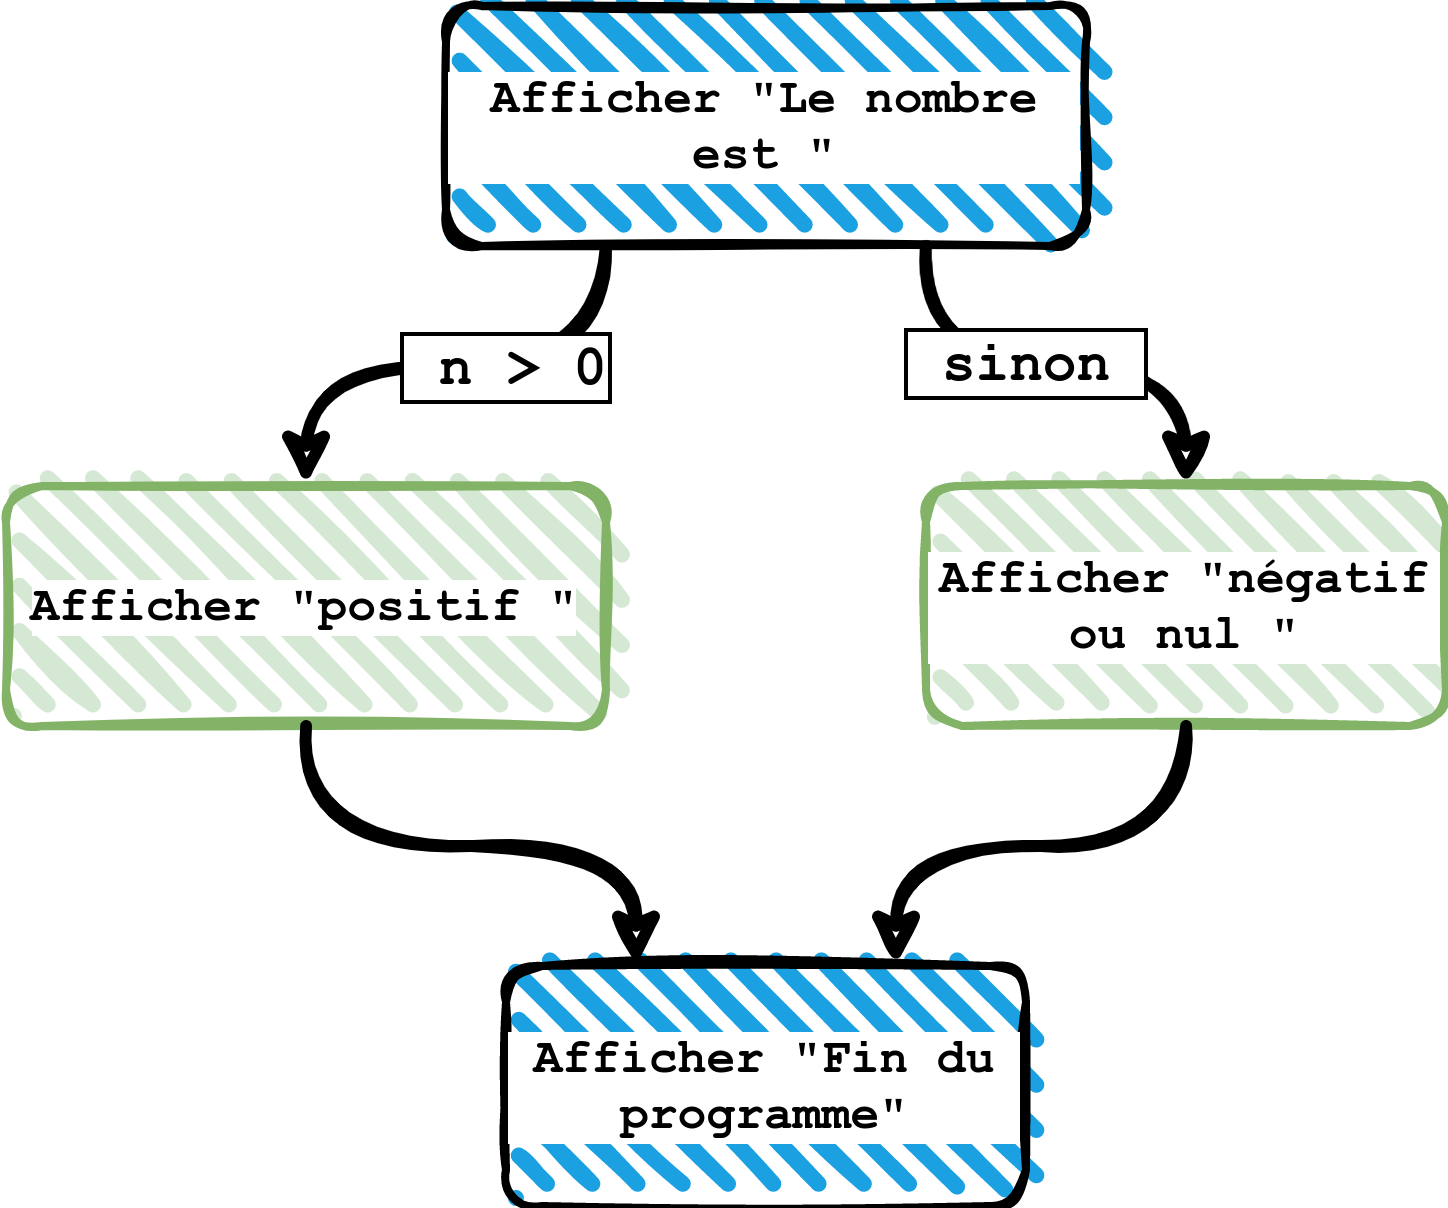
\includegraphics{res/branche02.png}
\caption{diagramme}
\end{figure}

    \hypertarget{trois-branches-ou-plus}{%
\paragraph{Trois branches ou plus}\label{trois-branches-ou-plus}}

    Enfin, il est possible d'introduire trois branches ou plus. Après un
premier test avec le mot-clé \texttt{si}, chaque branche suivante peut
être ajoutée avec \textbf{sa propre condition}.

Pour cela on utilise en pseudo-code le mot clé \texttt{sinon\ si} qui
est traduit en Python par \texttt{elif}.

Ce mot-clé est suivi d'une condition terminée par le symbole \texttt{:}.
\begin{exemple}
    \textbf{Pseudo-code}

\begin{verbatim}
si n < 0:
    afficher "Négatif"
sinon si n = 0:
    afficher "Nul"
sinon si n <= 2:
    afficher "Petit"
sinon:
    afficher "Grand"
\end{verbatim}

\textbf{Python}

\begin{Shaded}
\begin{Highlighting}[]
\ControlFlowTok{if}\NormalTok{ n }\OperatorTok{\textless{}} \DecValTok{0}\NormalTok{:}
    \BuiltInTok{print}\NormalTok{(}\StringTok{"Négatif"}\NormalTok{)}
\ControlFlowTok{elif}\NormalTok{ n }\OperatorTok{==} \DecValTok{0}\NormalTok{:}
    \BuiltInTok{print}\NormalTok{(}\StringTok{"Nul"}\NormalTok{)}
\ControlFlowTok{elif}\NormalTok{ n }\OperatorTok{\textless{}=} \DecValTok{2}\NormalTok{:}
    \BuiltInTok{print}\NormalTok{(}\StringTok{"Petit"}\NormalTok{)}
\ControlFlowTok{else}\NormalTok{:}
    \BuiltInTok{print}\NormalTok{(}\StringTok{"Grand"}\NormalTok{)}
\end{Highlighting}
\end{Shaded}

        \end{exemple}
    \begin{figure}
\centering
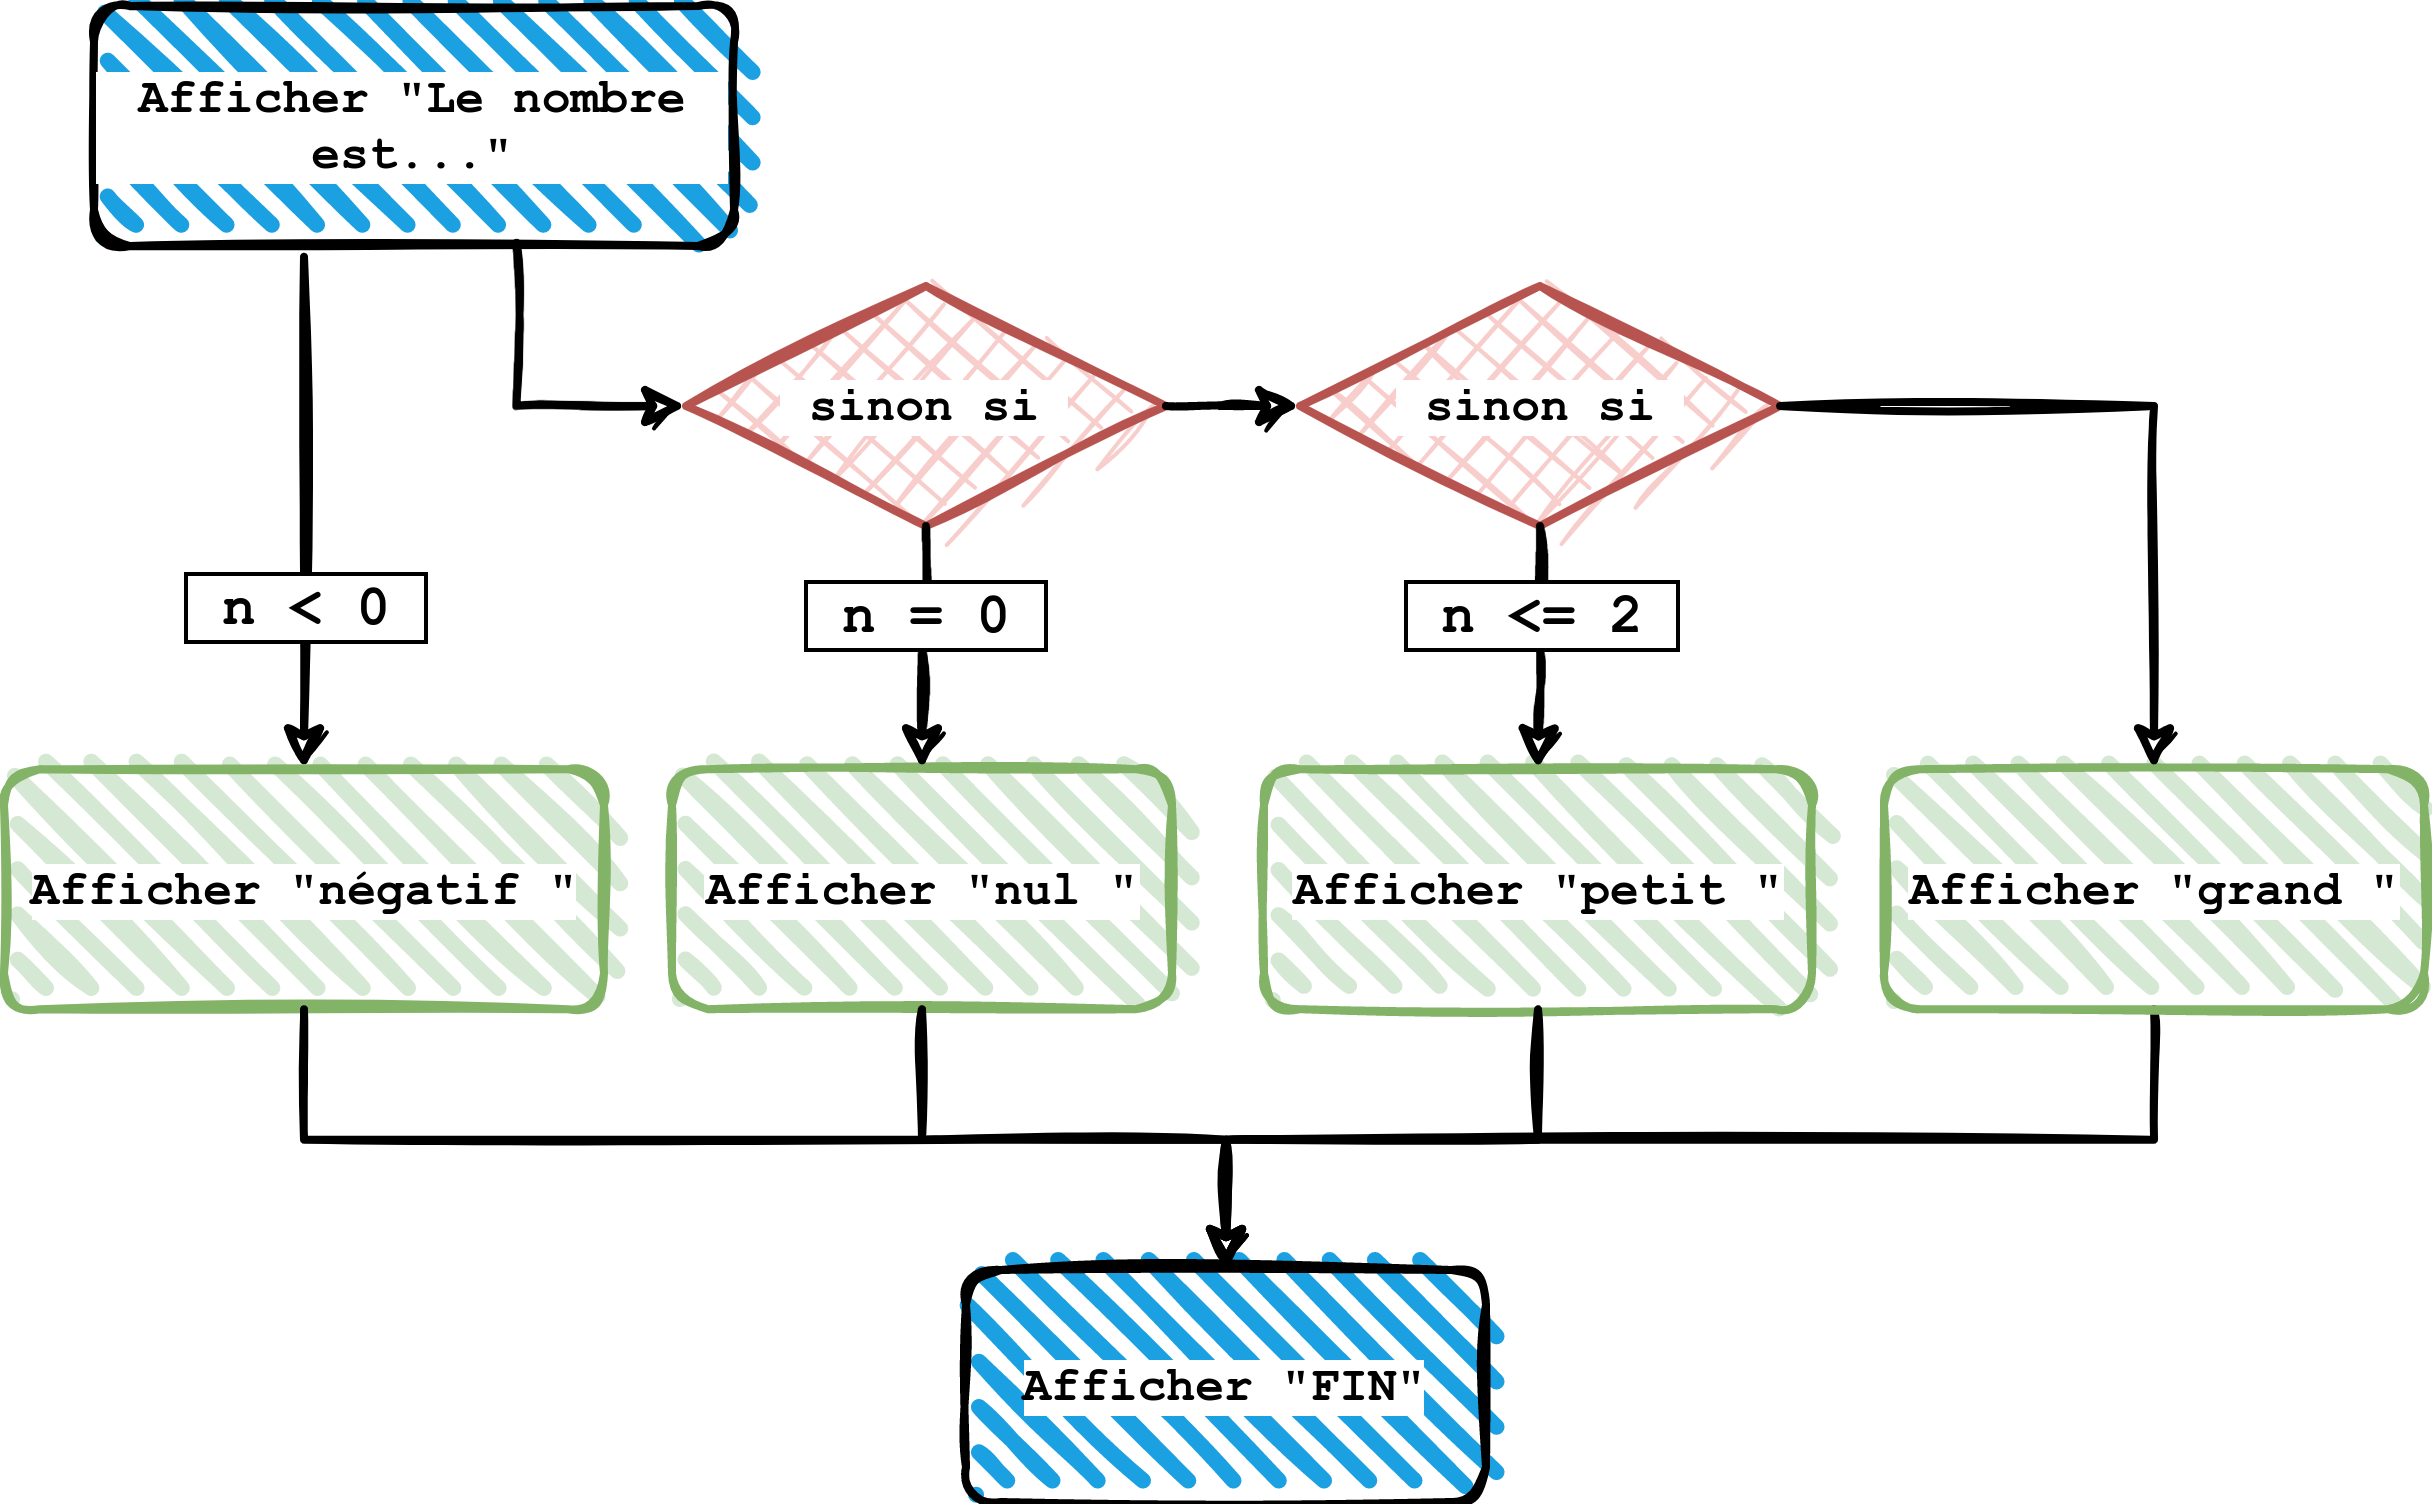
\includegraphics{./res/branche01.png}
\caption{Diagramme}
\end{figure}
\begin{remarque}
    Remarquez bien que l'\textbf{ordre} dans lequel apparaissent les
conditions est important.

        \end{remarque}\begin{remarque}
    Les opérateur de comparaison (tout comme on l'a vu \texttt{+} et
\texttt{*}) s'utilisent \textbf{aussi} avec \textbf{autre chose} que les
nombres !

Python compare les chaînes en fonction de l'\textbf{ordre
lexicographique}.

Exemples :

\begin{itemize}
\tightlist
\item
  \texttt{"abcd"\ \textless{}\ "b"} est une condition qui est
  \texttt{Vrai}
\item
  \texttt{"123"\ \textless{}\ "13"} est une condition qui est
  \texttt{Vrai}
\item
  attention aux majuscules : \texttt{"Z"\ \textless{}\ "a"} est
  \texttt{Vrai}
\item
  attention aux accents : \texttt{"wagon"\ \textless{}\ "été"} est
  \texttt{Vrai}
\end{itemize}

        \end{remarque}\begin{retenir}
    Attention, on ne peut pas comparer une \textbf{chaîne de caractère} et
un nombre \textbf{entier} ou un \textbf{flottant}.

        \end{retenir}\begin{eleve}
    Au bowling, on a deux chances pour faire tomber un total de dix quilles.
Écrire un algorithme qui demande le nombre de quilles renversées avec
chacune des deux boules et affiche \texttt{"X"} si toutes les quilles
sont tombées à la première boule, \texttt{"/"} si toutes les quilles
sont tombées, et sinon le nombre de quille renversées.

Exemples :

\begin{verbatim}
>>> Score première boule : 2
>>> Score deuxième boule : 3
5

>>> Score première boule : 7
>>> Score deuxième boule : 3
/

>>> Score première boule : 10
>>> Score deuxième boule : 0
X
\end{verbatim}
        
        \end{eleve}
    \hypertarget{expressions-booluxe9ennes}{%
\subsubsection{6.3 Expressions
booléennes}\label{expressions-booluxe9ennes}}

    Les \emph{conditions} sont des expressions algorithmique ordinaire qui
produisent un résultat. On les appelle des \textbf{expressions
booléennes}.

Une expression booléenne admet deux résultats possibles :

\begin{longtable}[]{@{}ll@{}}
\toprule
pseudo-code & \texttt{vrai} ou \texttt{faux}\tabularnewline
\midrule
\endhead
Python & \texttt{True} ou \texttt{False}\tabularnewline
\bottomrule
\end{longtable}
\begin{exemple}
    Par exemple, l'expression booléenne \(10 < 5\) est évaluée par
l'algorithme et produit le résultat \texttt{faux}.

Ainsi les deux pseudo-code suivant sont équivalent et n'affichent jamais
rien :

\begin{verbatim}
# algo 1
si 10 < 5:
    afficher "jamais"
    
# algo 2
si faux:
    afficher "jamais"
\end{verbatim}

        \end{exemple}\begin{retenir}
    Il est possible de faire des opérations avec les expressions booléennes
grâce à trois \textbf{opérateurs} :

\begin{itemize}
\tightlist
\item
  \texttt{et}, appelé la \emph{conjonction}
\item
  \texttt{ou}, appelé la \emph{disjonction}
\item
  \texttt{non}, appelé la \emph{négation}
\end{itemize}

        \end{retenir}\begin{exemple}
    Par exemple, prenons deux expressions booléennes \(e_1\) et \(e_2\),
alors :

\begin{longtable}[]{@{}ll@{}}
\toprule
\begin{minipage}[b]{0.47\columnwidth}\raggedright
\(\big( e_1 \texttt{ et } e_2 \big)\) est une expression booléenne
\texttt{vraie}\strut
\end{minipage} & \begin{minipage}[b]{0.47\columnwidth}\raggedright
si et seulement si \(e_1\) est \texttt{vraie} et \(e_2\) est
\texttt{vraie}\strut
\end{minipage}\tabularnewline
\midrule
\endhead
\begin{minipage}[t]{0.47\columnwidth}\raggedright
\(\big( e_1 \texttt{ ou } e_2 \big)\) est une expression booléenne
\texttt{vraie}\strut
\end{minipage} & \begin{minipage}[t]{0.47\columnwidth}\raggedright
si et seulement si \(e_1\) est \texttt{vraie} ou \(e_2\) est
\texttt{vraie}\strut
\end{minipage}\tabularnewline
\begin{minipage}[t]{0.47\columnwidth}\raggedright
\(\big( \texttt{non } e_1 \big)\) est une expression booléenne
\texttt{vraie}\strut
\end{minipage} & \begin{minipage}[t]{0.47\columnwidth}\raggedright
si et seulement si \(e_1\) est \texttt{fausse}\strut
\end{minipage}\tabularnewline
\bottomrule
\end{longtable}

        \end{exemple}
    Les opérateur booléens permettent donc de combiner plusieurs tests de
comparaison et d'égalité \textbf{en une seule expression}.
\begin{exemple}
    Par exemple l'algorithme suivant compare les coordonnées
\texttt{(xa,\ ya)} et \texttt{xb,\ yx)} de deux points \(x\) et \(y\) et
affiche des informations sur leurs positions relatives.

\[
\begin{array}{ll}
\text{si $x_a = x_b$ et $y_a = y_b$ :} \\
\qquad\text{afficher "points confondus"} \\
\text{sinon si $x_a = x_b$ ou $y_a = y_b$ :} \\
\qquad \text{afficher "points alignés horizontalement ou verticalement"}\\
\text{sinon :}\\
\qquad\text{afficher "points indépendants"}
\end{array}
\]

ce qui se traduit en Python par :

\begin{Shaded}
\begin{Highlighting}[]
\ControlFlowTok{if}\NormalTok{ xa }\OperatorTok{==}\NormalTok{ xb }\KeywordTok{and}\NormalTok{ ya }\OperatorTok{==}\NormalTok{ yb:}
    \BuiltInTok{print}\NormalTok{(}\StringTok{"points confondus"}\NormalTok{)}
\ControlFlowTok{elif}\NormalTok{ xa }\OperatorTok{==}\NormalTok{ xb }\KeywordTok{or}\NormalTok{ ya }\OperatorTok{==}\NormalTok{ yb:}
    \BuiltInTok{print}\NormalTok{(}\StringTok{"points alignés horizontalement ou verticalement"}\NormalTok{)}
\ControlFlowTok{else}\NormalTok{:}
    \BuiltInTok{print}\NormalTok{(}\StringTok{"points indépendants)}
\end{Highlighting}
\end{Shaded}

        \end{exemple}\begin{remarque}
    \textbf{Priorité des opérateurs booléens} Comme pour les expressions
arithmétiques, on a établit des conventions de priorité :

la négation est \textbf{plus prioritaire que} la conjonction qui est
\textbf{plus prioritaire que} la disjonction.

L'expression \[\text{$a$ ou non $b$ et $c$}\] doit être comprise comme
\[\text{$a$ ou $\big(($non $b$) et c$\big)$ .}\]

Mais, \textbf{il ne faut pas hésiter à mettre des parenthèses} pour
faciliter la lecture !

        \end{remarque}\begin{remarque}
    \textbf{Paresse des opérateurs booléens en Python}

\textbf{conjonction :} L'expression booléenne \texttt{e1\ and\ e2} n'est
vraie que si \texttt{e1} est vraie et \texttt{e2} est vraie. Ainsi,
\textbf{il suffit que} \texttt{e1} soit fausse pour que l'expression
complète soit fausse, et ceci, sans même avoir à évaluer l'expression
\texttt{e2} !

Et c'est exactement ce que fait l'interprète Python : il tente d'éviter
d'évaluer une expression si le résultat final est déjà connu. Dans notre
exemple, l'interprète fonctionne ainsi :

\begin{enumerate}
\def\labelenumi{\arabic{enumi}.}
\tightlist
\item
  évaluer \texttt{e1}
\item
  si \texttt{e1} est \texttt{faux} alors la conjonction vaut
  \texttt{faux}
\item
  sinon, évaluer \texttt{e2} (et la conjonction à la même valeur que
  \texttt{e2})
\end{enumerate}

        \end{remarque}\begin{exemple}
    Par exemple, imaginons un algorithme qui indique si un nombre \(a\) est
divisible par un nombre \(b\). Cette situation est caractérisée par le
fait que \(a\) vaut \(0\) ou que le reste de la division de \(a\) par
\(b\) vaut \(0\). Le reste s'obtient grâce à l'opérateur
\(a \text{ mod } b\) (appelé \emph{modulo} et qui se calcule en Python
en écrivant \texttt{a\ \%\ b})

Cependant, l'opérateur \emph{modulo} n'a pas de sens si \(b\) vaut \(0\)
(car on ne peut pas, mais \textbf{vraiment pas} diviser par \(0\) !!!!),
ce qui déclenche une erreur en Python.

Ainsi, la condition complète pour savoir si \(a\) est divisible par
\(b\) sera donc :

\begin{itemize}
\tightlist
\item
  soit \(a = 0\) ;
\item
  soit \(b \neq 0\) \textbf{et} \(a \text{ mod } b = 0\)
\end{itemize}

En l'écrivant ainsi dans un programme en Python, l'évaluation paresseuse
du \textbf{et} évite l'évaluation problématique de \(a \text{ mod } b\)
lorsque \(b\) vaut 0.

Algorithme correct :

\[
\begin{array}{ll}
\text{si $a=0$ ou $\big( b \neq 0$ et $a$ mod $b = 0 \big):$}\\
\qquad \text{afficher "divisible"}\\
\text{sinon:}\\
\qquad \text{afficher "pas divisible"}
\end{array}
\]

Algorithme incorrect qui engendre une erreur en Python lorsque \(b=0\):

\[
\begin{array}{ll}
\text{si $a=0$ ou $\big( a$ mod $b = 0$ et $b \neq 0\big)$}\\
\qquad \text{afficher "divisible"}\\
\text{sinon:}\\
\qquad \text{afficher "pas divisible"}
\end{array}
\]

        \end{exemple}\begin{eleve}
    Implémenter un programme qui demande deux nombres à l'utilisateur et
affiche \texttt{"divisible"} si le premier est divisble par le second et
qui affiche \texttt{"pas\ divisible"} sinon.
        
        \end{eleve}

    % Add a bibliography block to the postdoc
    
    
    
\end{document}
